\chapter{System Design}
\label{chap:systemDesign}

This chapter discusses the design of the application developed for this thesis. The aim is to develop a stand-alone desktop application to view and interact with out-of-core point clouds. The application offers various methods for the user to interact with the point cloud. The application has three main elements that work together, all controlled by the user. 

\par

Shape detection, as described in Chapter \ref{chap:shapeDetection}, is performed on a sub-region of the point cloud one at a time. Section \ref{sec:user_guided_sd} describes an interactive heuristic that selects an octree node as a region of interest, using the user's cursor position and camera view as input. Using the user's input effectively changes the task of detecting shapes from an automated approach to a user-controlled interaction.

\par

Most interactions presented in this thesis share similar techniques and naming conventions. Therefore, some terms that are used throughout this chapter are defined in Section \ref{sec:termDefinitions}. 

\par

Section \ref{sec:shapePicking} describes a picking algorithm to select a primitive shape from the screen that can later be used as support shape for assisted user interactions. 

\par

Section \ref{sec:interactions} provides detailed information on the additional user interactions that use a support shape as assistance. \textit{point picking, region selection}, and textit{local level-of-detail increment} are all interactions that benefit from the use of a support shape. 


\section{Term Definitions}
\label{sec:termDefinitions}

The basis of all interactions is the user's cursor on the screen. The \textit{pick ray} is a ray that origins from the cursor’s position in world space and goes in the direction of the camera to the cursor position. 
Each interaction iteratively filters the octree's data such that coarse filtering is carried out before finer adjustments are performed on the dataset before choosing a final candidate. Data that survives the coarse filtering is referred to as \textit{candidate}, e.g., candidate nodes or candidate points. 


\section{User-guided Shape Detection}
\label{sec:user_guided_sd}

The shape-detection algorithm is already described in Chapter \ref{chap:shapeDetection}. As the shape detection computation usually takes several minutes, the approach in this thesis performs this computation on small chunks of roughly the same size of point-cloud data at a time. The octree already provides the point cloud as pieces of spatially-neighboring data, such that each node describes an enclosed subset of the point cloud at a specific level-of-detail. Using chunks of the same size allows the user to expect results in about the same time for each node. This response time should ideally be a fraction of a second, at best less than $250$ milliseconds. 

The \textit{user-guided shape detection} is updated continuously in the background, relying only on the user's current mouse position and view. Thus, only nodes are considered that intersect the pick ray. To be selected as candidate node from the octree, a node must fulfill the following constraints: 
\begin{enumerate}
    \item The node must currently be rendered and visible to the user. 
    \item The node must intersect the pick ray.
    \item The node must contain at least $n$ points, the same amount used as minimal support point count for shape detection.
    \item The node must not have been processed before. Hence, it already contains detected shapes. 
\end{enumerate}

These constraints have the following motivation: Since the user controls the shape-detection process, it makes sense that the user only interacts with what is presented on screen. Therefore, the node must currently be rendered and visible. To reduce the amount of redundant computation, only nodes that contain enough points to fit at least one shape are considered to be candidates. Lastly, the shape-detection algorithm works under the probabilistic assumption that, once it terminates, all shapes in this region are detected. Therefore, nodes that already contain detected shapes do not qualify as candidates as well. 

\par

The culling operation on the octree, described in Section \ref{sec:renderHorizon}, returns an octree that only contains nodes that are rendered. Thus, all nodes in this tree are already visible to the user and fulfill constraint 1. Only a single raycast with the pick ray needs to be performed on the culled octree to obtain the set of candidate nodes that fulfill constraints 1 and 2. 

\par

From this set, nodes are eliminated that do not fulfill constraints 3 and 4. The heuristic favors nodes with higher level-of-detail, such that the user receives geometric information for the most detailed parts of the currently explored region first. The projected distance to the nearplane is used to select between nodes with the same level of detail. The node closest to the camera is chosen. 

\par

The selection of a suitable candidate node depends heavily on the camera position. When zooming out, the camera moves away from the scene, thus reducing the render horizon and therefore reducing the maximum level-of-detail. If the node with the highest level of detail is processed already the heuristic chooses a node from a lower level of detail. Thus, a multi-scale representation of the local geometry is constructed over time, creating a level of detail for primitive shapes as well. 


\section{Shape Picking}
\label{sec:shapePicking}

This thesis presents several interactions that are supported by using detected shapes to ease interactions with point clouds. The use of a support shape raises the need for an initial interaction to pick a primitive shape. A raycast is performed on the culled octree using the pick ray to create an initial filtering of octree nodes. From this set of nodes only those shapes are collected that intersect the pick ray. The picking heuristic prefers primitive shapes of higher level of detail that are closer to the camera. All primitive shapes are collected from the candidate nodes and sorted using a custom key. Primitive shapes that intersect the pick ray come with information on the nearest intersection point and the level of detail. For each intersection point, the $depth$ in range of $[0,1]$, where $0$ is at the near plane and $1$ is at the far plane, is calculated. For shapes that have more than one intersection points, the intersection point closest to the camera is chosen. The sort key is composed as follows: 

$$key = level + 1 - depth$$.

The primitive shape with the highest key is chosen as support shape. The composition of the key ensures that a shape with the highest level of detail that is closest to the camera is picked. 

\par

As a primitive shape only covers a small region, limited by the extents of the octree node, and user interactions are usually performed on larger areas, a single primitive shape is not sufficient to provide semantic information to the user. Therefore, once a shape is picked, a cluster is created from this shape using primitive shapes that are similar to this shape. This clustering is described in Section \ref{sec:shapeClustering} in depth. All shapes are collected from visible nodes that match the picked shape. From this set of shape a coherent cluster is created, such that each shape has a neighbor within $\epsilon$ distance, as described in Chapter \ref{chap:shapeDetection}. A cluster can be seen as a single, multi-level shape and is referred to as \textit{support shape}.


\section{Shape-Assisted Interactions}
\label{sec:interactions}

Creating new interactions is a key topic in this thesis. In 3D applications, classic two-dimensional interaction metaphors, such as \textit{lasso selection} and \textit{point picking}, are limited by the lack of information on the desired depth. In a 3D setting,  these interactions must either guess the desired depth boundaries or ignore them. Furthermore, these interactions lack the possibility to mask out unwanted points from a selection. Unwanted points are selected on a regular basis. Hence, many view changes are necessary to select only points that are of interest. Using a primitive shape as support, the user can easily interact with the point cloud in a way that only points are considered that belong the support shape. 

\par

Figure \ref{fig:interaction_workflow} shows the basic workflow for shape-assisted user interaction. The workflow comprises two major steps. The first interaction is to pick a primitive shape and build a larger cluster from it. This cluster acts as a support shape for the following user interaction. For this interaction, when initialized, all affected nodes are collected and their point sets are filtered to only those points that are approximated by this shape. Hereby, a point is filtered if it fulfills the same $\epsilon$-distance and normal-deviation criteria in regards to the support shape as used for the shape detection in Chapter \ref{chap:shapeDetection}. After the filtering step, the actual interaction is performed on the remaining points. 

\par

Sections \ref{sec:pointPicking} and \ref{sec:regionSelection} describe the pros and cons of current state-of-the-art two-dimensional interactions and propose improvements using the workflow mentioned earlier. Furthermore, Section \ref{sec:lod_increment} proposes a technique to locally increment the visible level of detail along structures of interest to amplify details. 


\begin{figure}
	\centering
	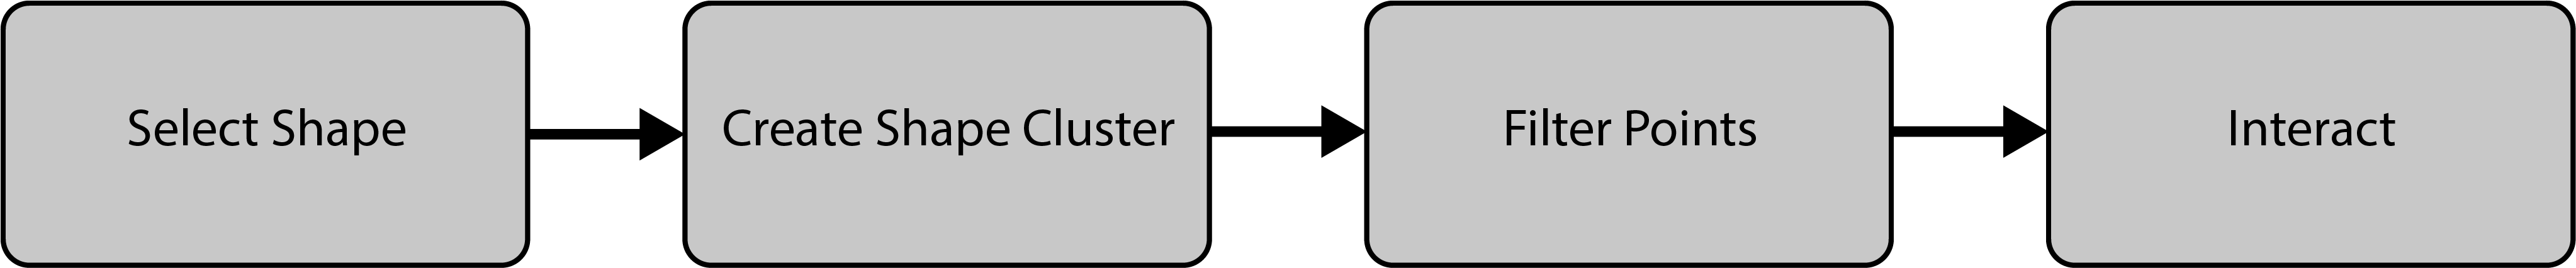
\includegraphics[width=0.8\textwidth]{System_Design/interaction_workflow.png}%7
	\caption[Workflow of an assisted user interaction]
	{The workflow for shape-assisted interactions is divided into two major steps. First, the user picks a primitive shape, from which a larger cluster is created and used as support shape for the following interaction. Upon starting an assisted interaction, the system finds all nodes that are affected by the interaction, reduces the set of points to those that are approximated by this shape and, finally, the interaction (e.g., selection, picking) is performed. }
		\label{fig:interaction_workflow}
\end{figure}
	

	
\subsection{Point Picking}
\label{sec:pointPicking}

\textit{Point Picking} describes an interaction where the user is interested in selecting a single point from the scene at a time. The pick radius $r$ denotes the maximum distance of a point to the pick ray for the point to be considered a candidate point. Multiple picking techniques influence the pick radius $r$ differently. The pick radius $r$ can either be constant in world space, constant in screen space or is depended on the depth value. This section gives two examples on how different pick radii influence the consistency of the picking interaction. After that, shape-assisted point picking is discussed as counterpart to the classic two-dimensional point picking. 


\subsubsection{Point picking in world space}

The first explored technique is to use a fixed pick radius in world space. The picked point is the point closest to the pick ray in world space. Since the user only interacts with points that are projected onto the near plane, the projection of the pick radius is smaller for points that lie in the background. Therefore, the distance in pixels from the mouse position to the picked point in the background is smaller than the distance to a picked point in the foreground. While this encourages the picking of points in the front, the non-uniform pixel distance introduces inconsistencies as the cursor reacts stronger to points in the foreground. 

\par

Using a simple raycast is not sufficient enough to find all octree nodes that are affected by this interaction. If the pick ray does not intersect the node's bounding box, it is still possible that the cylinder, created by the pick ray and the radius intersects the octree node. Hence, a cylindrical cast must be performed in order to collect all candidate nodes. 


\subsubsection{Point picking in screen space}

A more consistent way of picking a point is to only use the screen-space information for each point. The mouse position $p$ in screen space combined with the pick radius $r$ create the pick circle $c$. This circle corresponds to the projection of a cone in world space with it's apex at the camera position, the pick ray as direction and the opening angle defined by the pick radius. All points that intersect this cone are treated as candidate points. To calculate this intersection, all points are projected to the screen space. The cone intersects a point if $c$ contains the point in screen space. Then the point with the projection closest to the mouse position is picked. This technique works consistently for different depth values. However, since all points are treated equally, the method does not distinguish between foreground and background points, thus introducing possible depth ambiguities. 

\par

The projection of points can be executed on the GPU by rendering the projected points, paired with an identifier, to a texture. From this texture, a window around the mouse cursor is downloaded, and the closest point is determined. Reading pixels from a texture forces the CPU and GPU to sync and stalls the graphics pipeline. 

\par

Much like picking in world space, the complete set of candidate nodes cannot be retrieved by a simple raycast, as this means that some nodes are node considered that are would intersect the pick cone. Instead, a cone cast is performed to retrieve all affected octree nodes. This conecast is realized by projecting the corners of the node's bounding box onto the near plane, and calculating the convex hull polygon. The intersection is determined by the intersection of the polygon with the pick circle in screen space. 


\subsubsection{Shape-Assisted Point Picking}
\label {sec:picking_assisted}

Picking comes with the disadvantage that some constellations of points can influence the picking interaction negatively. The user is forced to change the view to pick an otherwise occluded point from the structure of interest. In some cases, a point in the background is favored over the desired point on a structure in the foreground. \textit{Shape-assisted point picking} utilizes primitive shapes to perform the picking routine only on points that are part of a structure. The user selects a cluster of shapes, thus reducing the number of possible candidate points to only those that belong to this support shape. 

\par

Rather than using a cone or raycast to collect all candidate nodes, only nodes whose bounding boxes intersect the support shape are considered. Furthermore, only points are considered that are approximated by the support shape. This reduction leaves only a handful of nodes and points that follow the curvature of the support shape on which the interaction is performed. 

\begin{figure}[p]
	\centering
	\subcaptionbox{ \label{fig:picking_raycast}}{%
		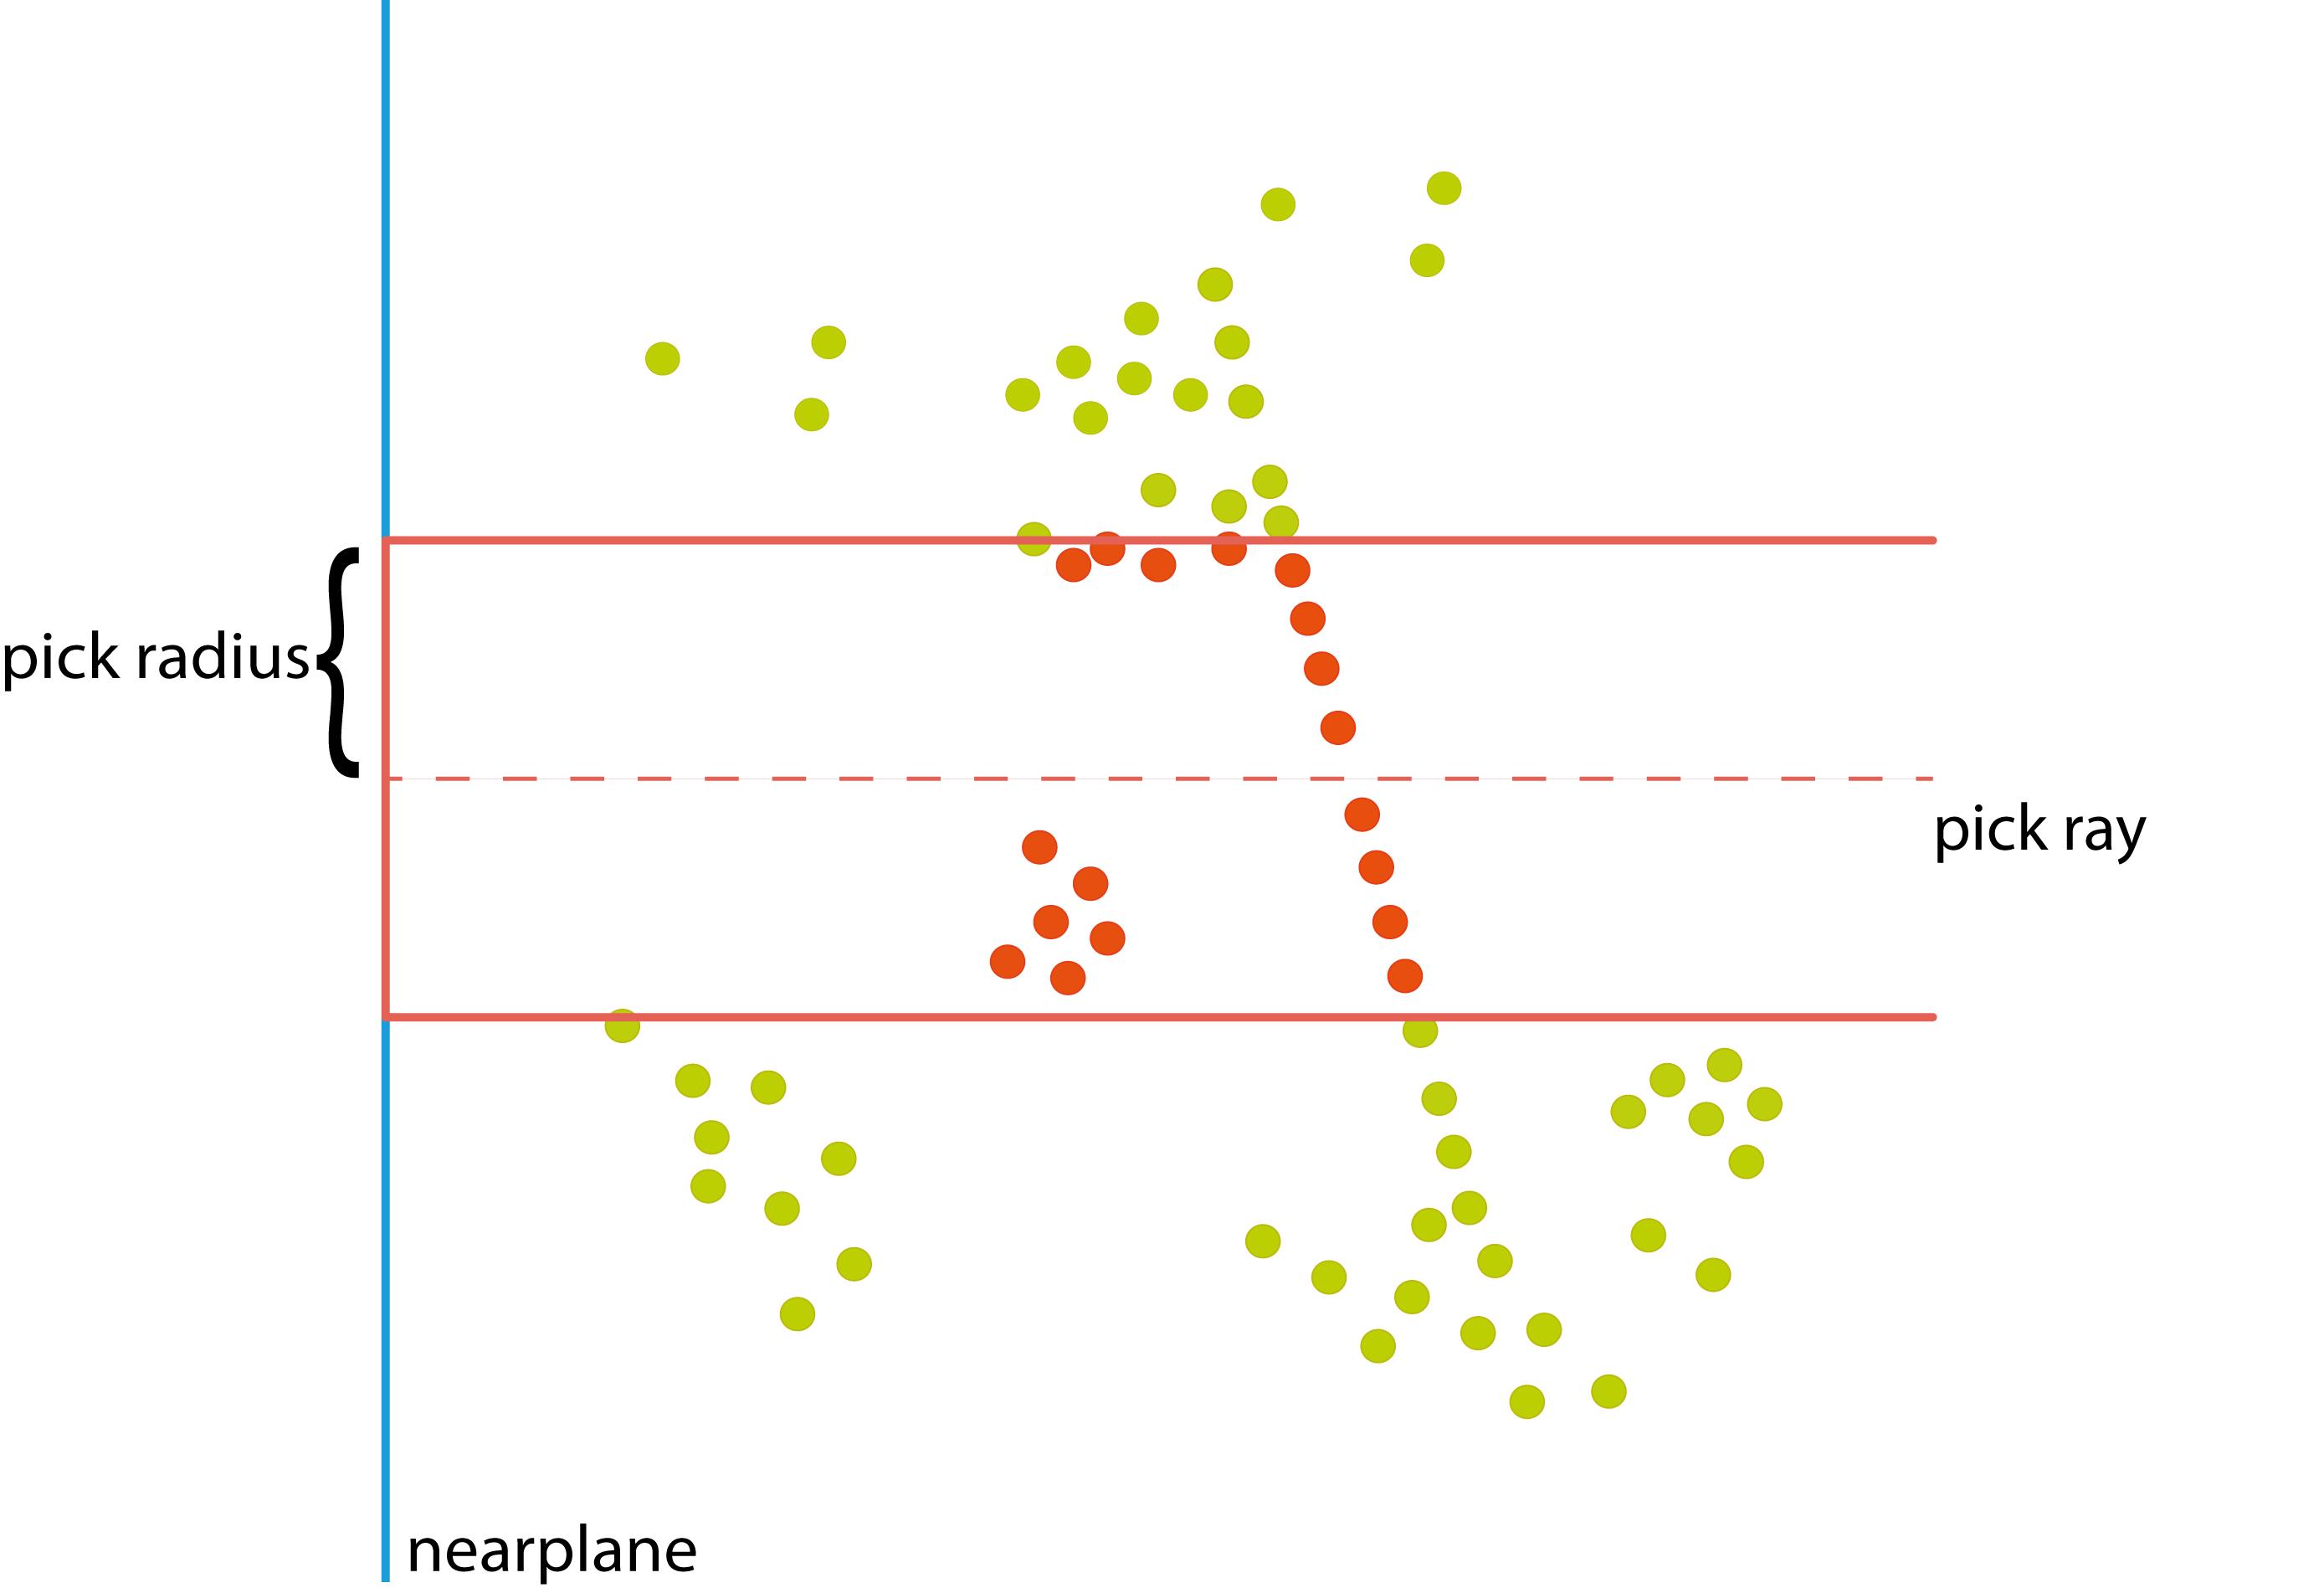
\includegraphics[width=0.6\textwidth]{System_Design/picking_raycast.png}%7
	}\par\medskip
	\subcaptionbox{ \label{fig:picking_conecast}}{%
		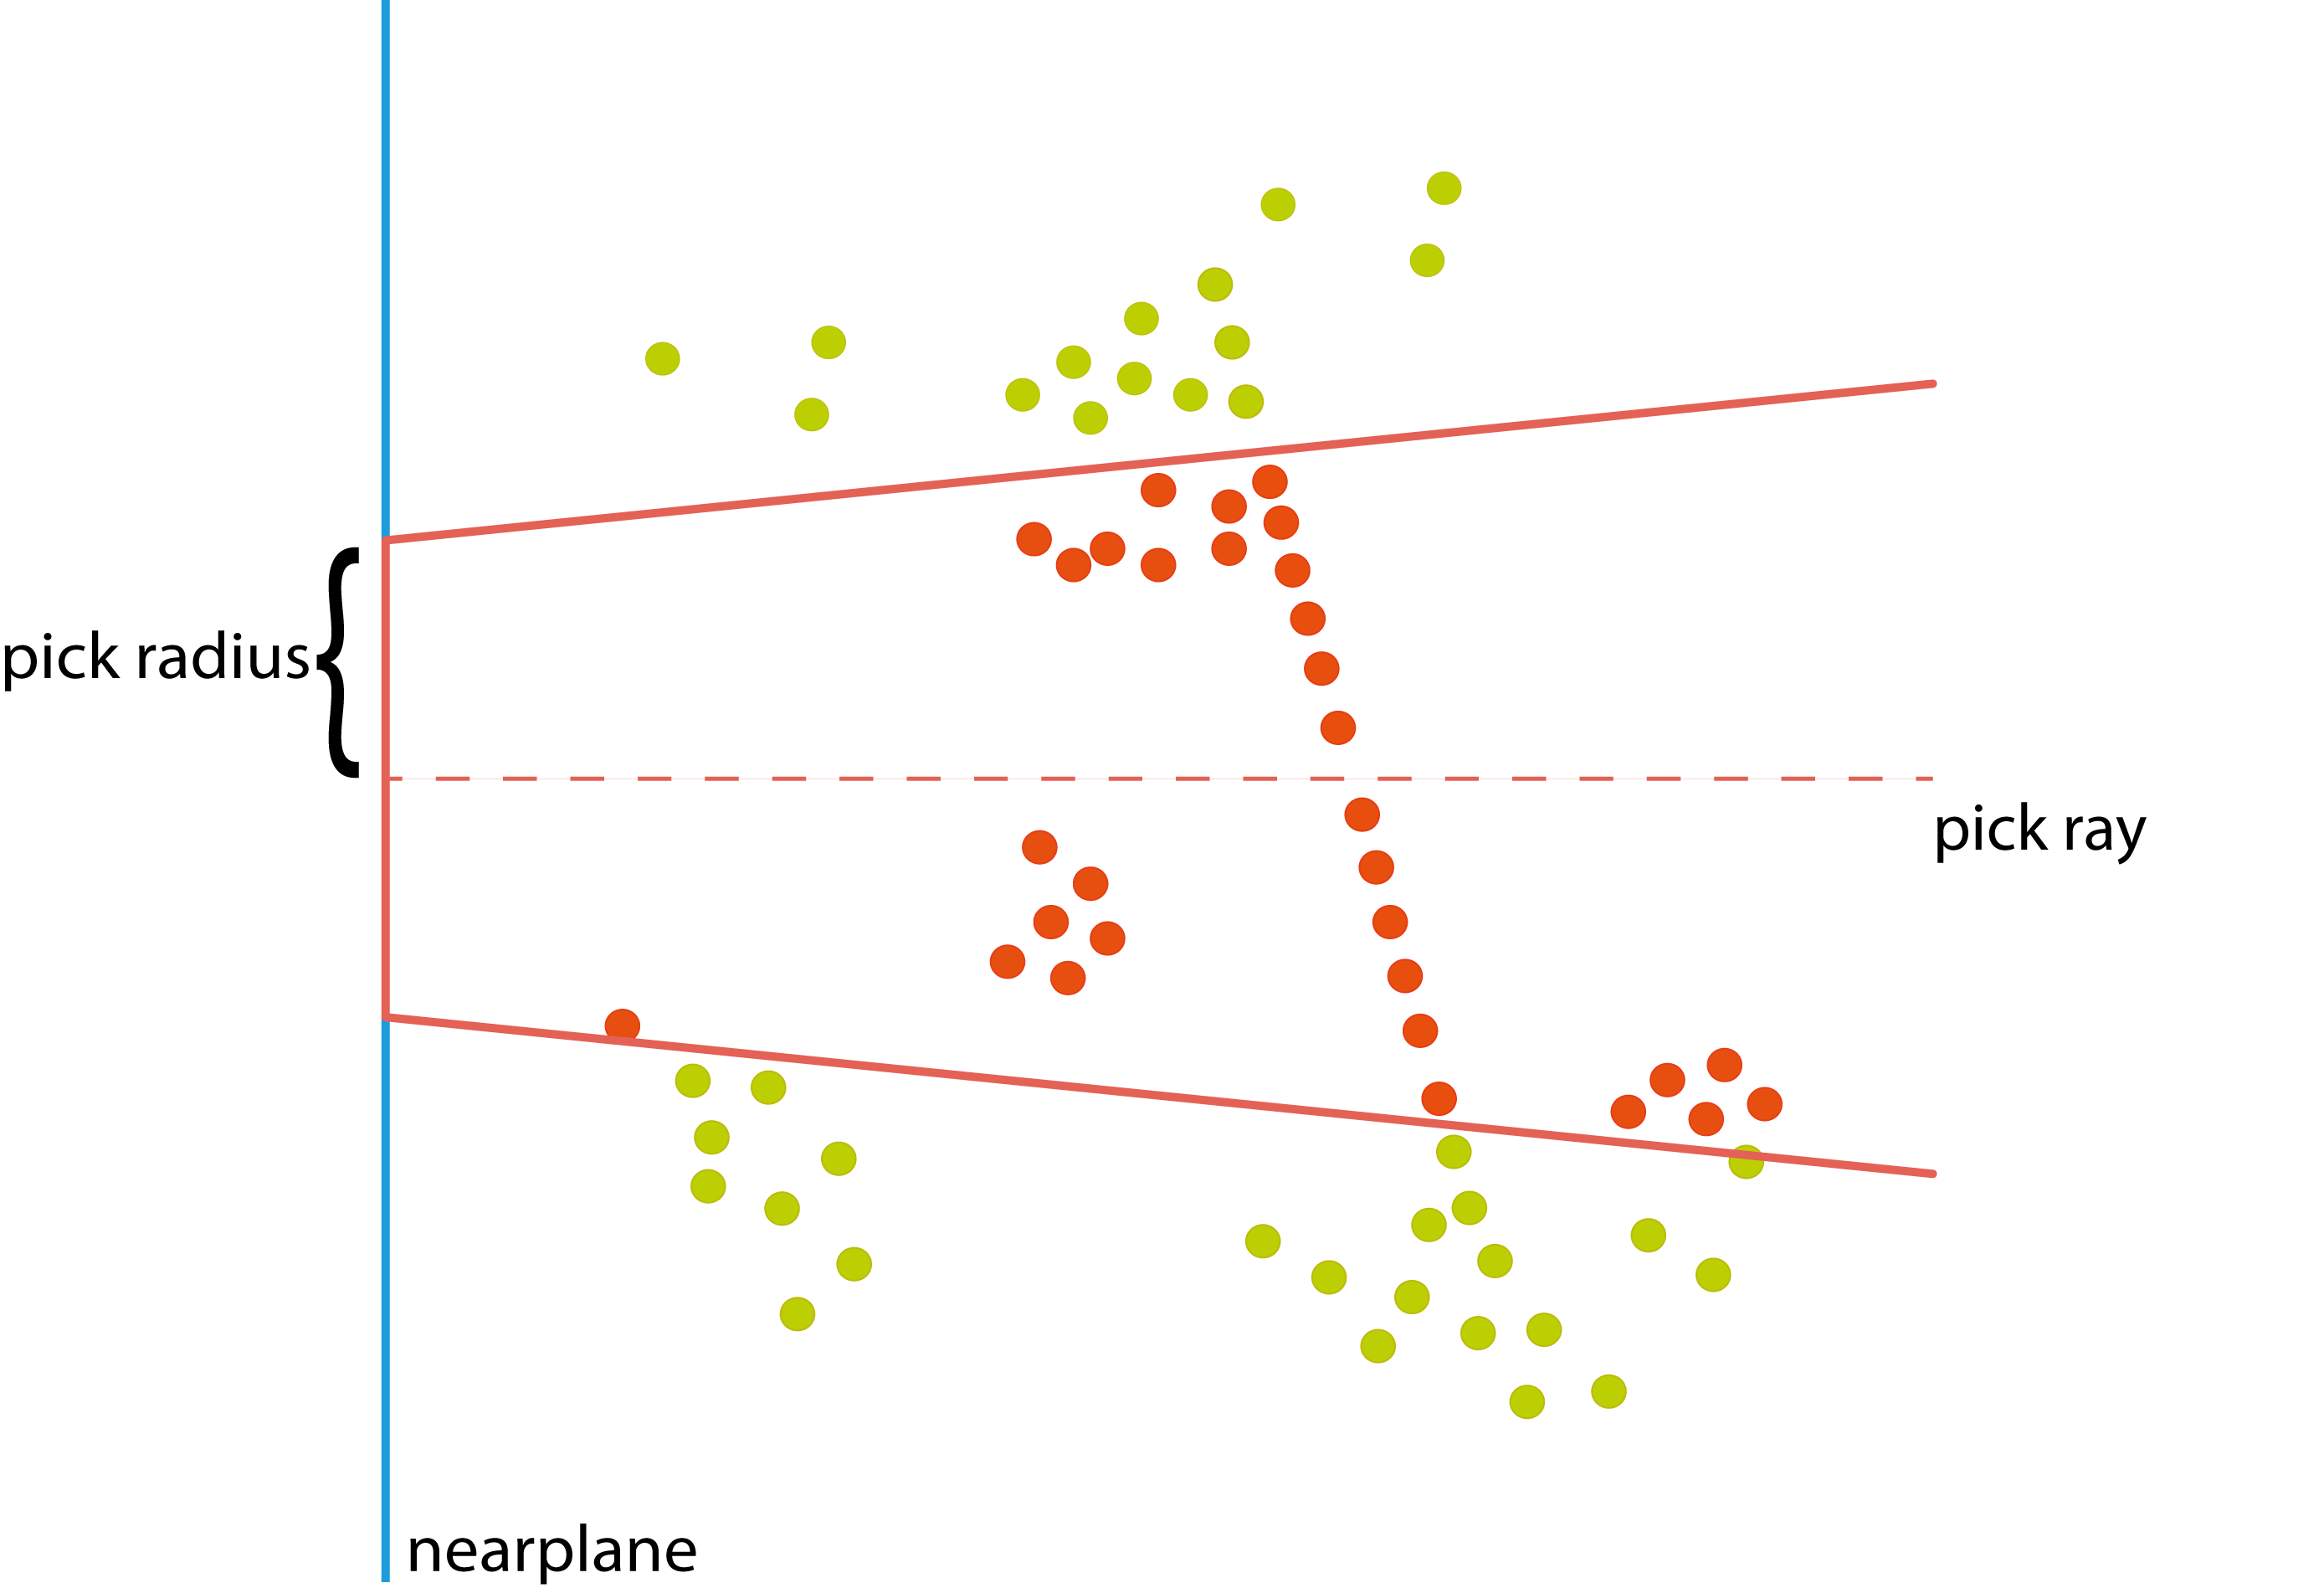
\includegraphics[width=0.6\textwidth]{System_Design/picking_conecast.png}%
	}\par\medskip        
	\subcaptionbox{ \label{fig:picking_assisted}}{%
		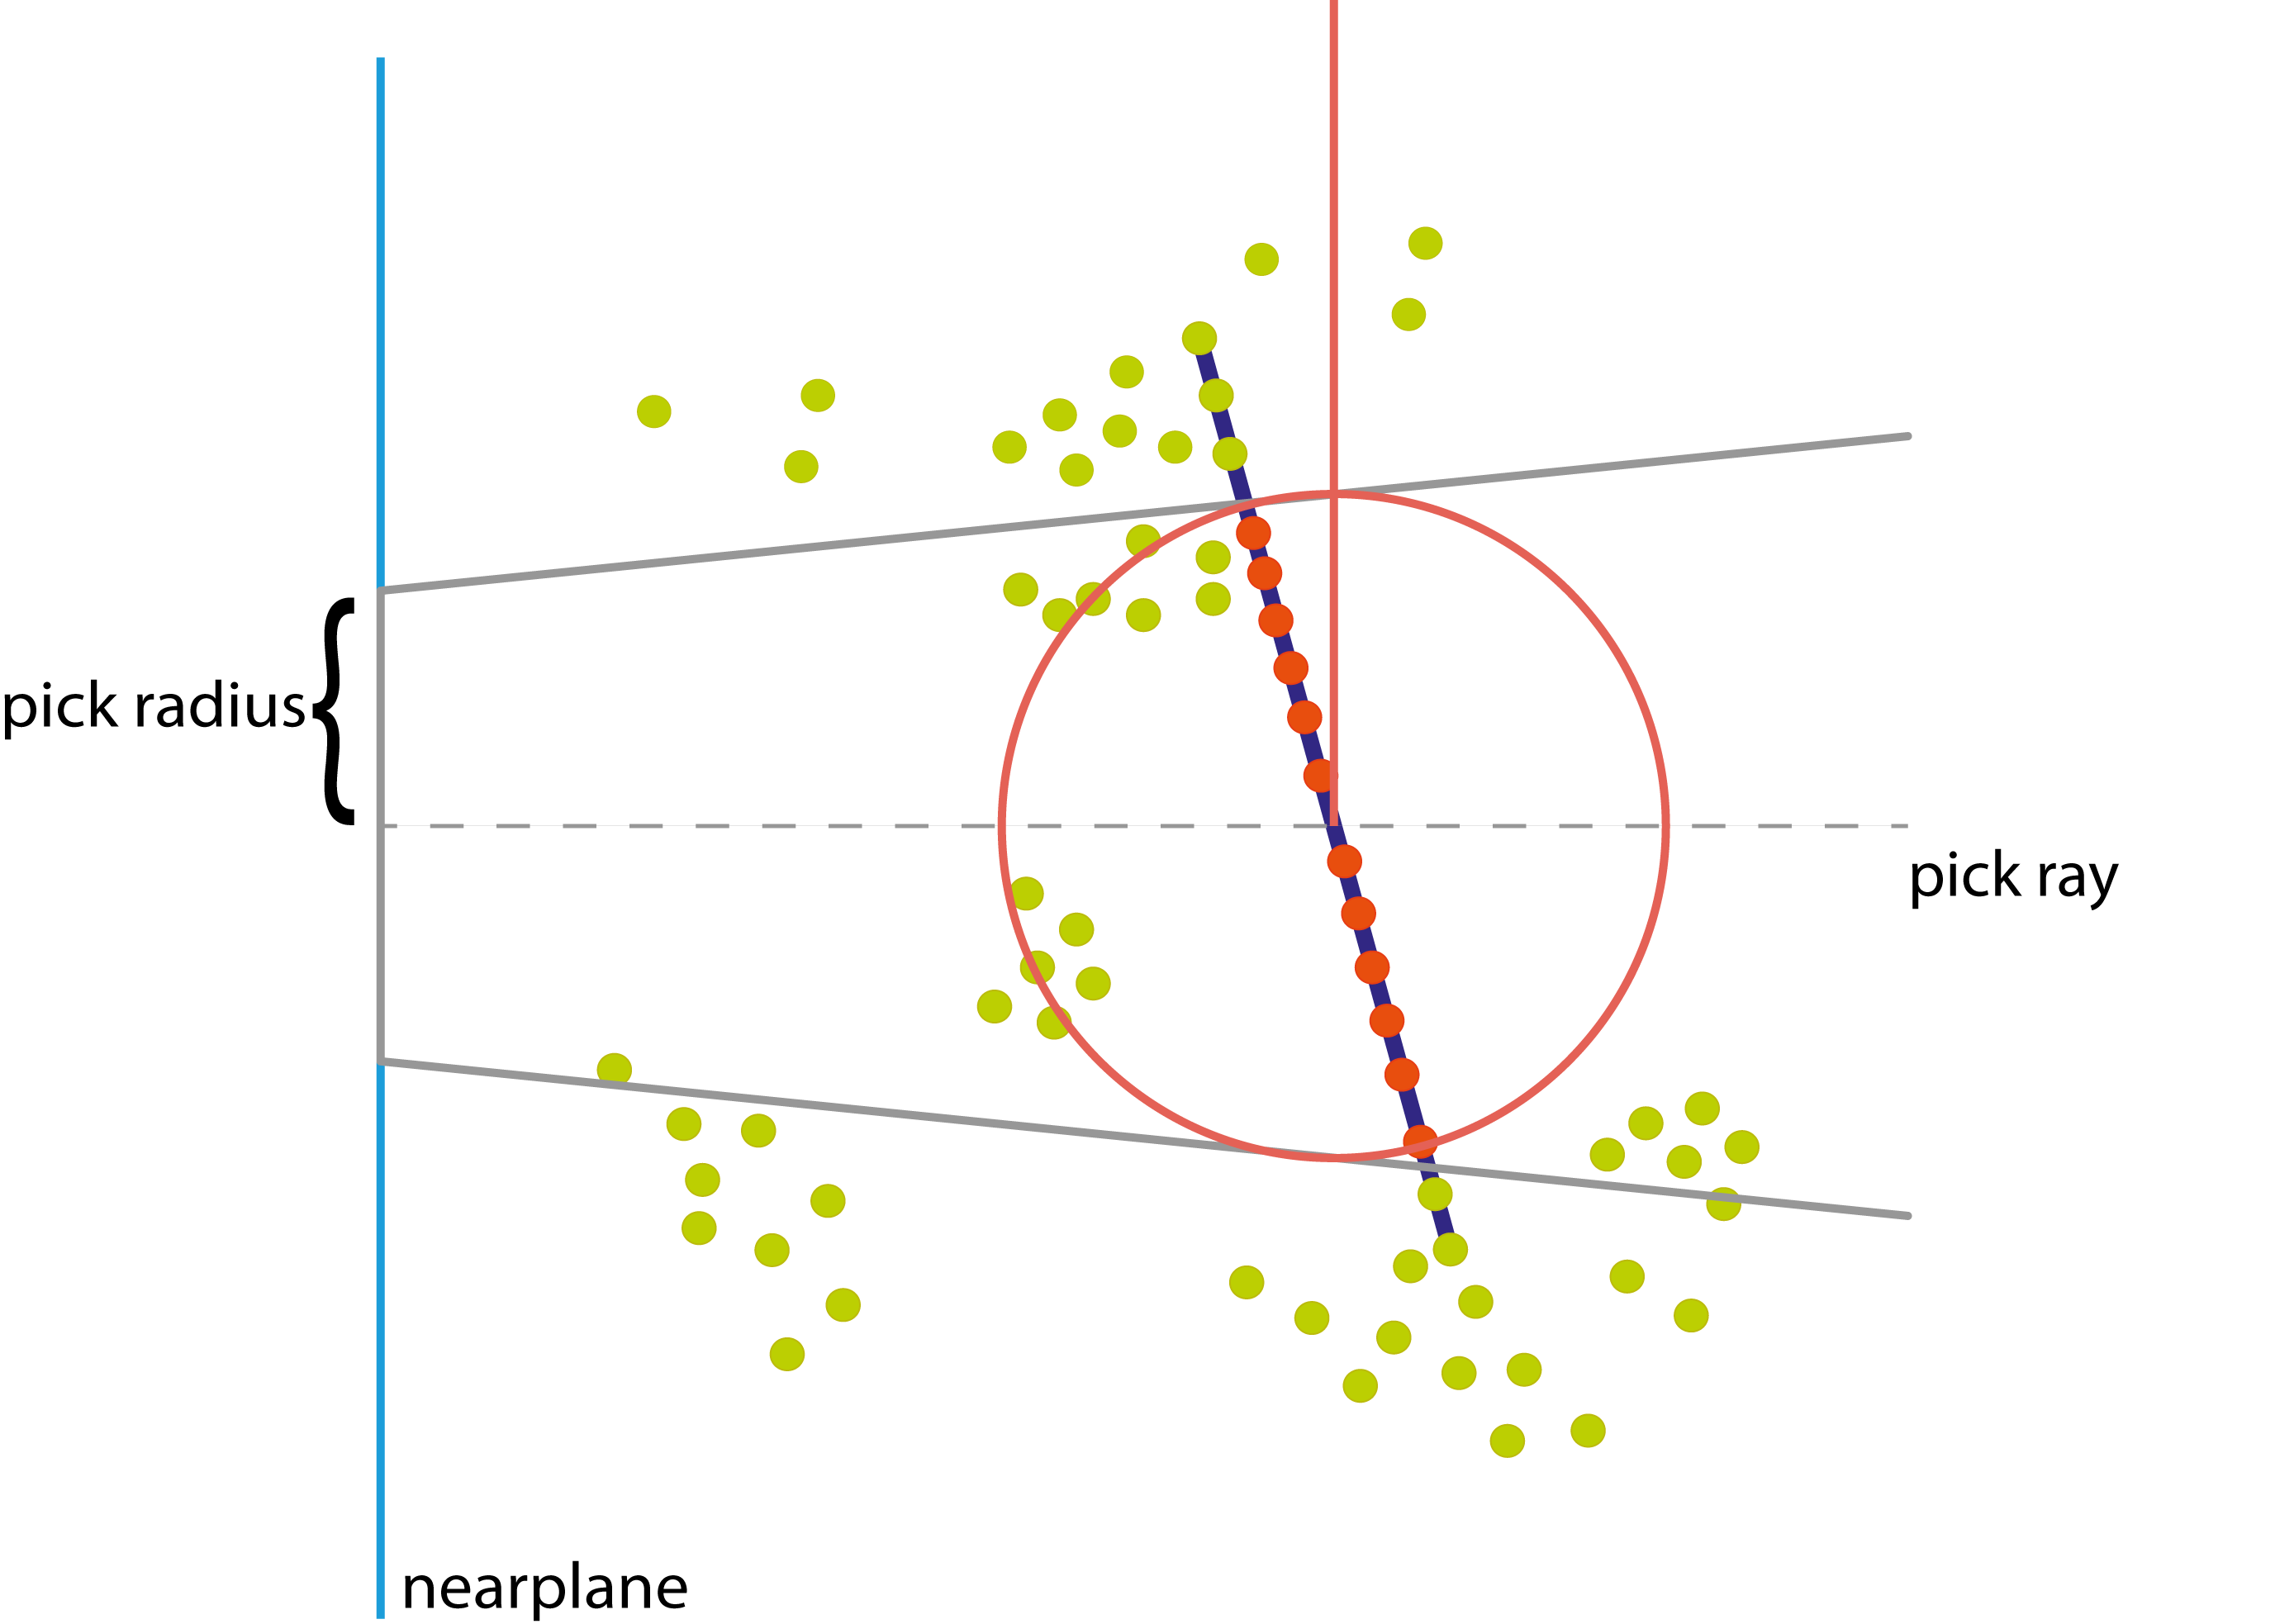
\includegraphics[width=0.6\textwidth]{System_Design/picking_assisted.png}%
	}
	\caption
	[Illustration on different picking methods. (a) shows a simple raycast, (b) a cone cast, (c) shows the use of a support shape combined with a sphere cast]
	{Two-dimensional illustration of various picking methods. Candidate points are colored in green; other points are colored in red. The areas in red describe the different volumes in which candidate points are located. (a) showcases a picking process using a simple raycast. The ray combined with a radius constructs a cylinder in world space that contains all candidate points, (b) uses a cone instead. (c) utilizes a selected shape (dark blue) to filter candidate points that follow the curvature of the shape. A sphere cast is then performed on the filtered points using the unprojected pick radius to obtain the final set of candidate points. }
	\label{fig:picking_overview}
\end{figure}

Due to shapes possibly having front and back sides, such as cylinders and spheres, points on the back of a shape are projected near the mouse position as well. By using the projected distances, points that lie on the back side of the shape might get favored over points that are on the front side of the shape (facing the user). Therefore, point picking is performed in world space using a pick sphere. The sphere's position is the intersection point of the pick ray with the support shape. The sphere's radius is calculated by unprojecting the pick radius to the intersection point. Only points are considered that lie in the pick sphere, constructed by the intersection point and the pick radius. The point closest to the intersection point is then selected. 

\par

This technique not only improves interaction; computation time is reduced as well. Usually, a shape cluster intersects fewer nodes than a raycast result as the cluster's extension is limited to a moderate region in the point cloud. The number of points per node is reduced as well, and distance measures are computed only for candidate points. 

\par

Figure \ref{fig:picking_overview} shows the different picking methods, described in Section \ref{sec:pointPicking}. Figure \ref{fig:picking_raycast} showcases a simple raycast with a radius. The combination of a ray and a radius yields a cylinder, which contains all candidate points on world space. The pick distance is consistent in world space. Figure \ref{fig:picking_conecast} uses a conecast instead. The opening angle is defined by the pick radius in screen space. The pick distance in world space increases the higher the depth value. All points inside the volume are treated equally, introducing consistency in screen space. Figure \ref{fig:picking_assisted} showcases the use of a support shape to filter candidate points. All points that belong to the support shape are filtered prior to being used as input for a spherecast. 

\begin{figure}
	\centering
	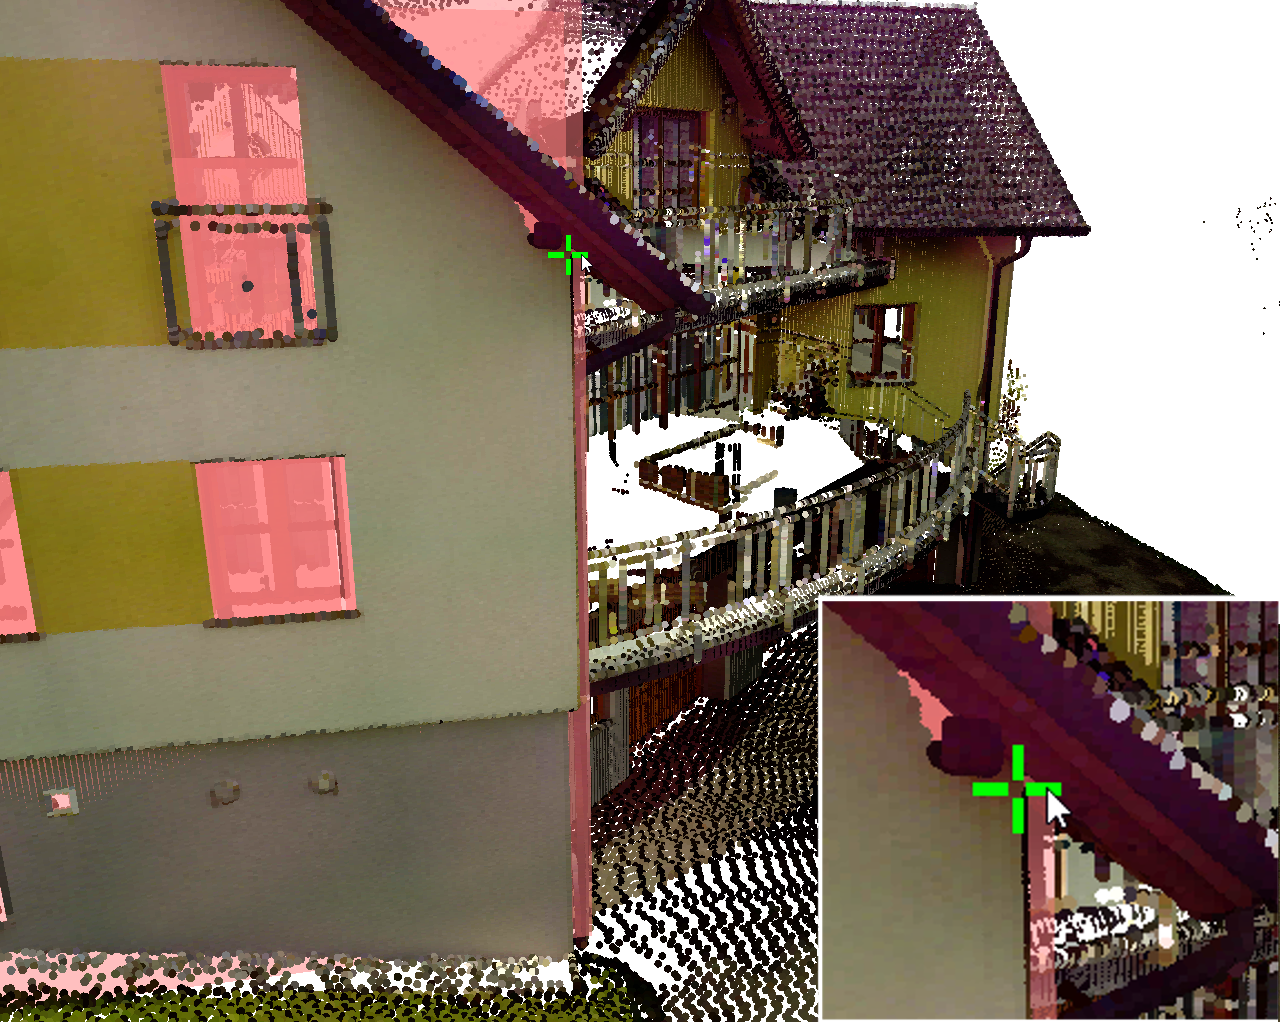
\includegraphics[width=0.8\textwidth]{System_Design/picking_assisted_screenshot.png}%7
	\caption[Screenshot of Shape-assisted Point Picking]
	{\textit{Shape-assisted point picking} is performed on a shape cluster that represents the wall in the foreground. The cross hair indicates the picked point. Note that the cross hair does not jump to a point in the background even though they would be closer to the cursor in screen space. }
	\label{fig:picking_assisted_screenshot}
\end{figure}

An example of \textit{shape-assisted point picking} can be seen in Figure \ref{fig:picking_assisted_screenshot}. The cross hair, even though other points' projections are closer to the cursor, sticks to the structure. Picking points on edges is improved in particular since the picking result follows the edge rather than jumping to a point in the background. 


\subsection{Region Selection}
\label{sec:regionSelection}

Region selection aims at selecting a set of points, that share certain criteria, rather than picking a single point. 
The design for the \textit{shape-assisted region selection} is guided by one seemingly simple example task: \textit{Select points that belong to this wall only}. A wall can intersect with other building elements such as roof, balconies or the ground. In regions close to intersections, it is tedious and cumbersome to only select points on the desired structure. Using two-dimensional interaction metaphors, selecting multiple spatially neighboring points along the same curvature is particularly challenging due to the system not knowing the desired depth boundaries for the selection region. In this section, the benefits of using support shapes for two- and three-dimensional interaction metaphors to select regions of points,  are discussed. 


\subsubsection{Lasso Selection}

The \textit{lasso selection} is a common two-dimensional interaction metaphor used for multiple geometry-based applications. While it is a useful technique to select regions in 2D, drawbacks appear when porting the interaction to 3D. The user draws a polygon onto the screen. All points whose projection lie inside this polygon are selected. Much like \textit{point picking}, points are projected onto the near plane, the intersection between the point and the lasso polygon in screen space determines whether or not a point is selected. The lasso polygon in combination with the camera view creates a three-dimensional volume, whose area contains all points whose projection lie inside the lasso polygon. Figure \ref{fig:lasso_sketch} showcases the volume created by a lasso polygon drawn onto the screen.

Note that this interaction is computed asynchronously and the selection is performed on the entire octree. Therefore, it is essential that octree nodes whose level-of-detail are too high and are therefore not rendered are still included in this interaction as well. 


\begin{figure}
	\centering
	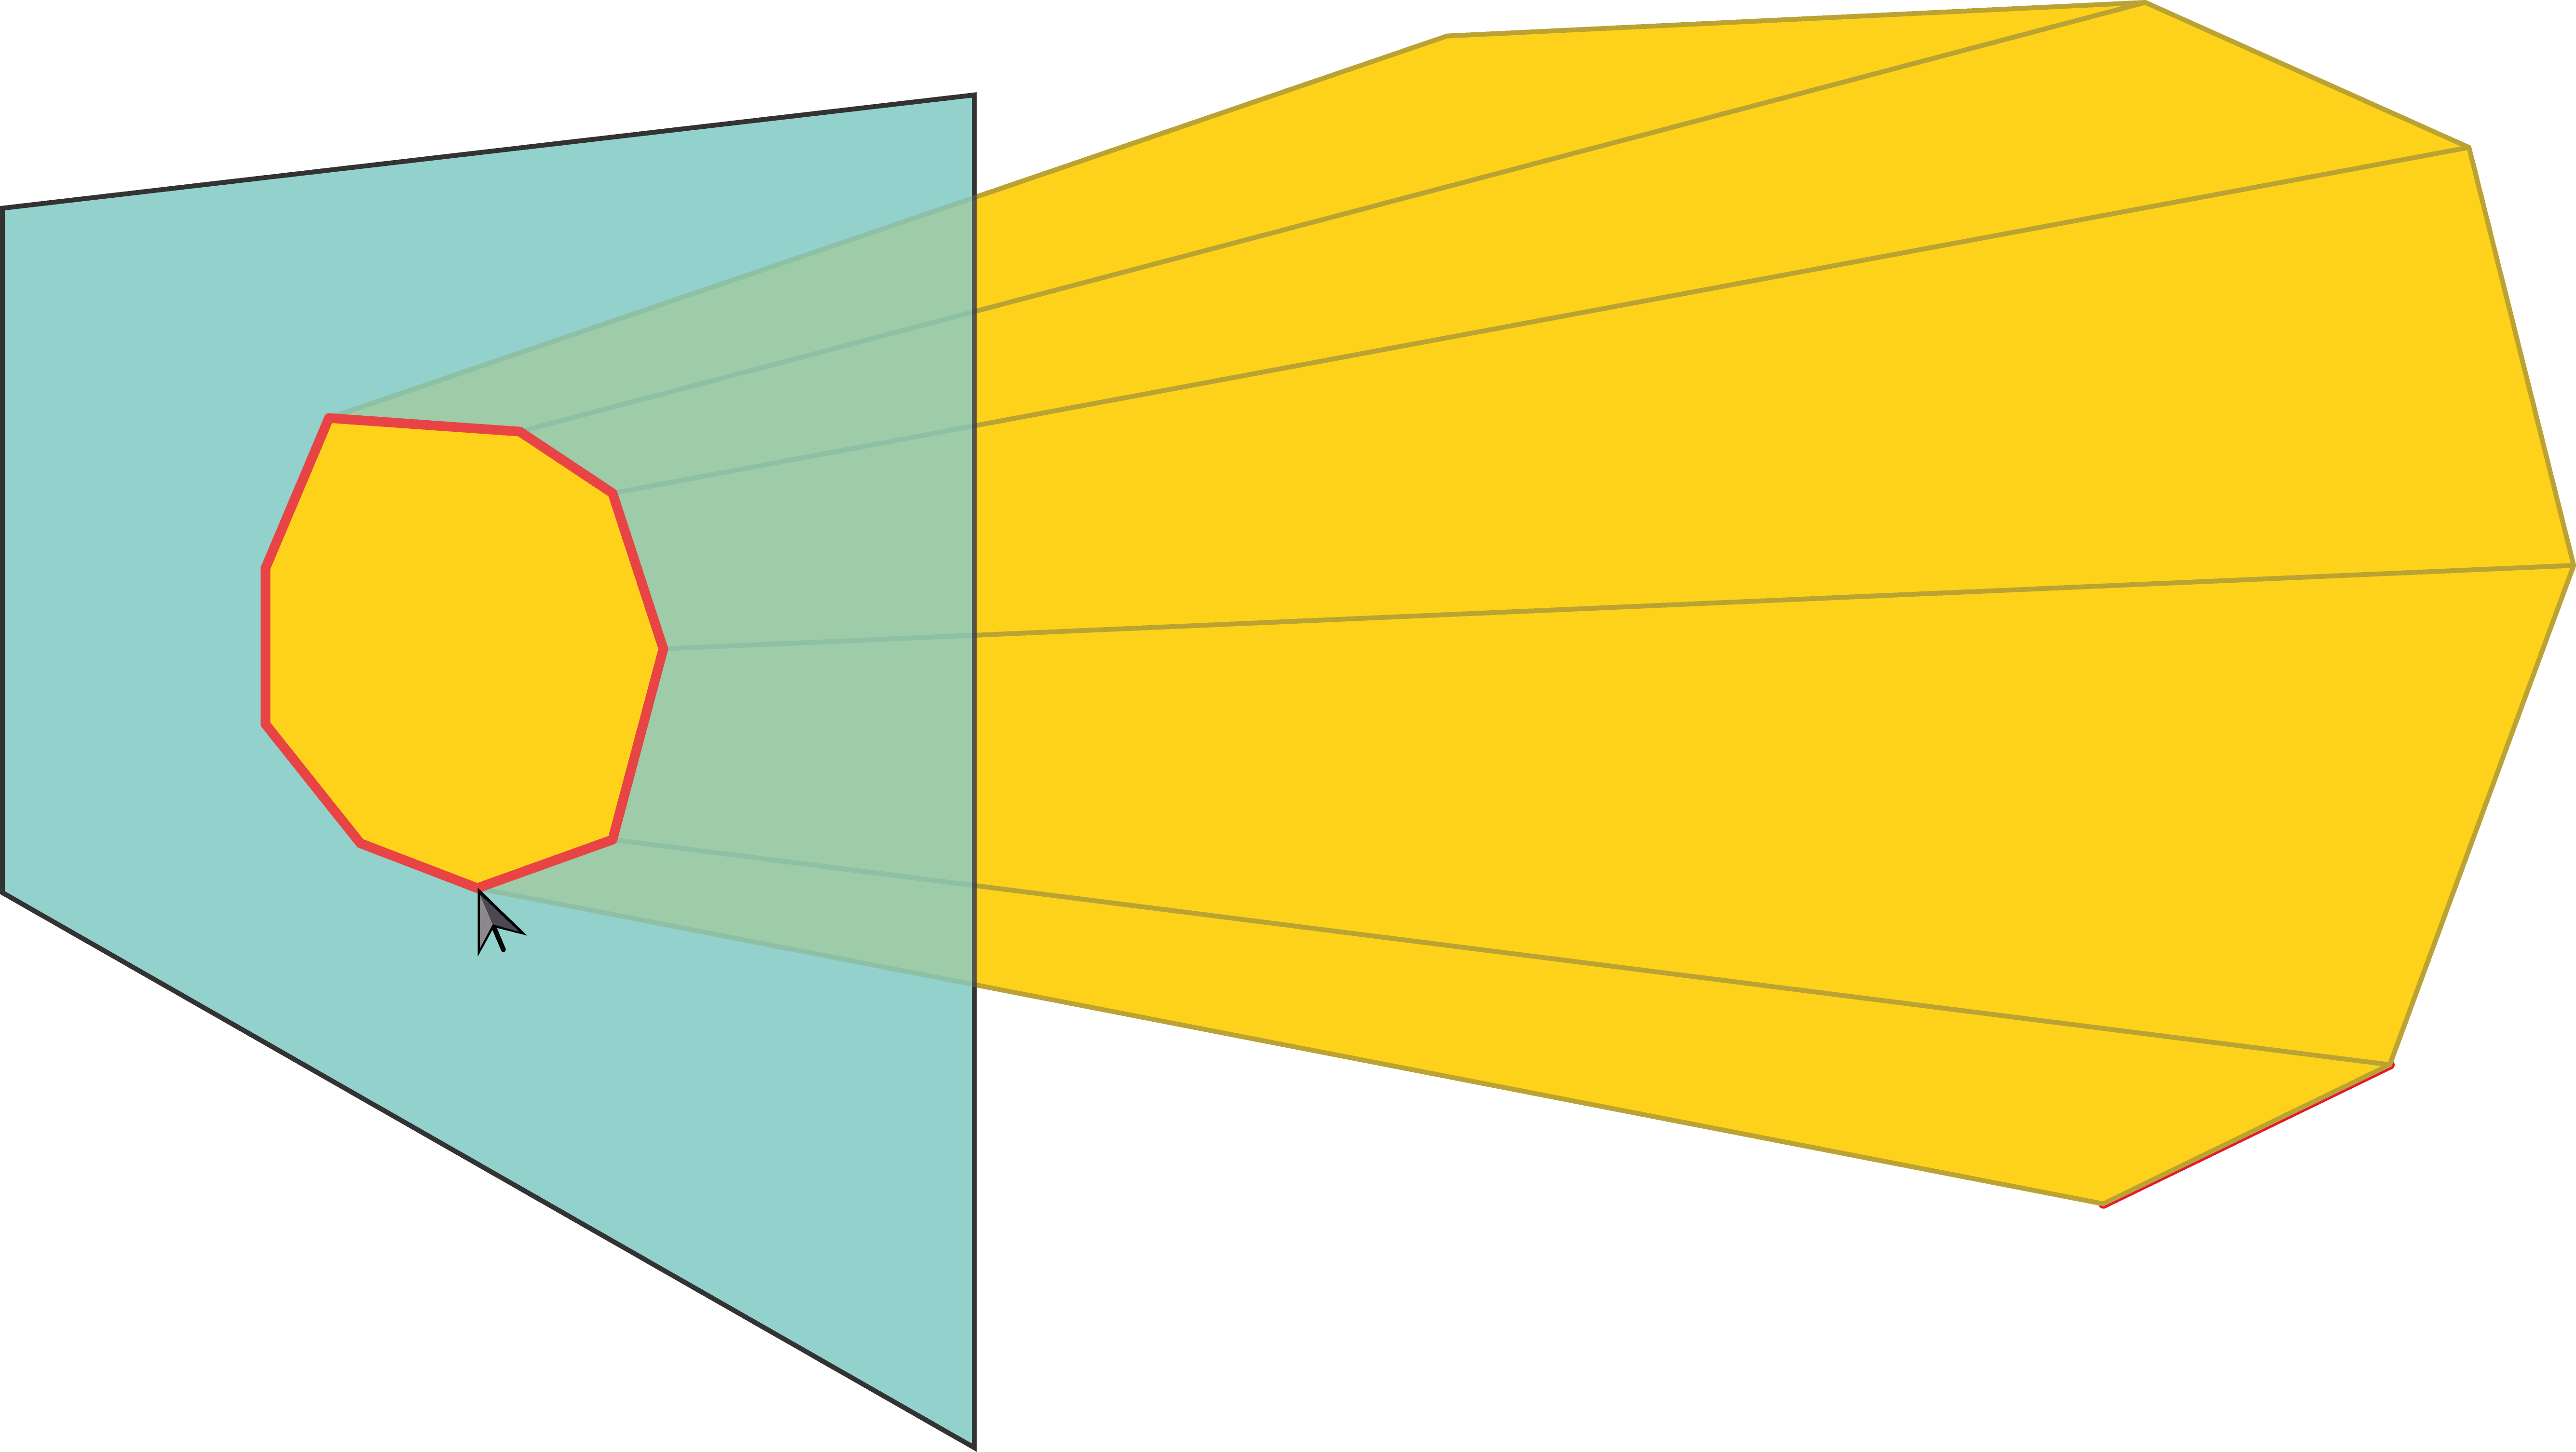
\includegraphics[width=0.8\textwidth]{System_Design/lasso_sketch.png}%7
	\caption[Illustration of the creation of a lasso selection]
	{The user draws a polygon (red) on the screen (light blue). The constructed three-dimensional area (yellow) contains all points whose projection lie inside the lasso polygon. }
	\label{fig:lasso_sketch}
\end{figure}


\begin{figure}
	\centering
	\subcaptionbox{ \label{fig:lasso1}}{%
		\includegraphics[width=0.5\textwidth]{System_Design/lasso1.png}%7
	}\par\medskip
	\subcaptionbox{ \label{fig:lasso2}}{%
		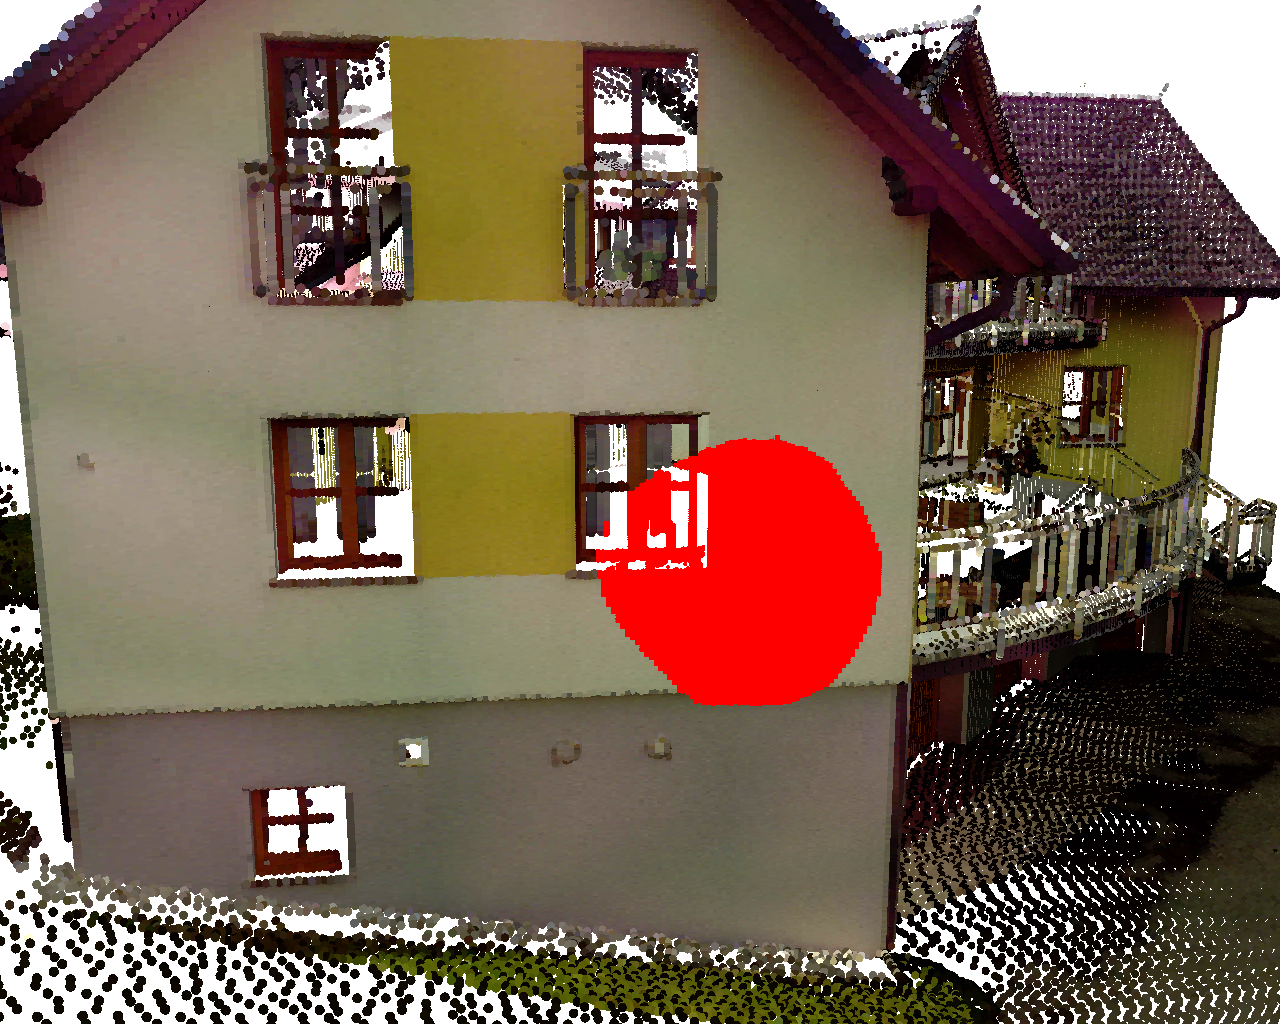
\includegraphics[width=0.5\textwidth]{System_Design/lasso2.png}%
	}\par\medskip        
	\subcaptionbox{ \label{fig:lasso3}}{%
		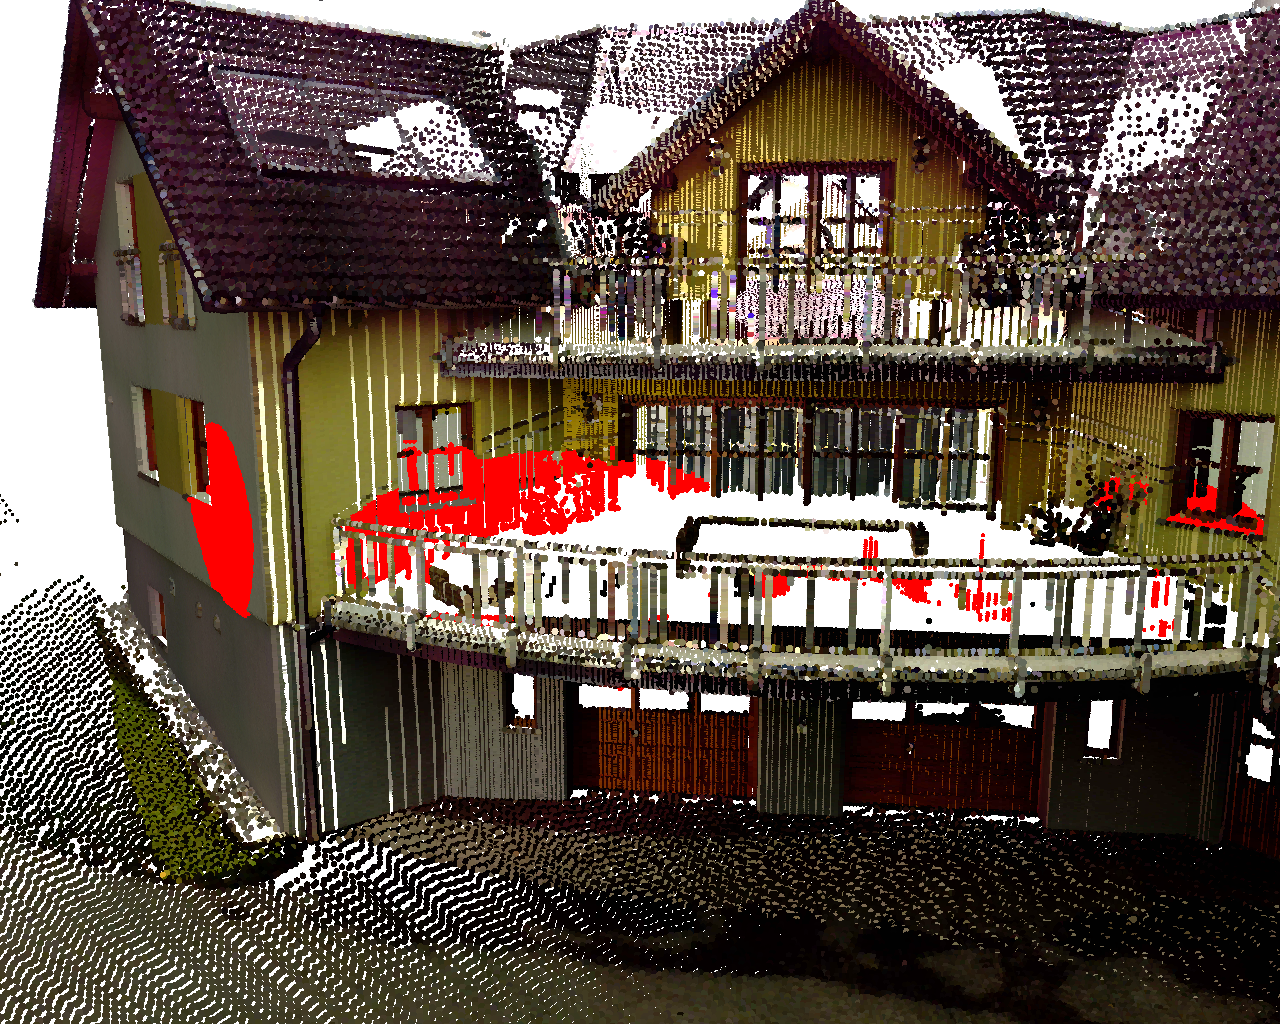
\includegraphics[width=0.5\textwidth]{System_Design/lasso3.png}%
	}
	\caption[Screenshots of the workflow of a lasso selection. (a) shows the lasso, (b) the selected points, (c) shows the selected points from a different angle. ]
	{(a) - (c) show a lasso selection performed on a point cloud. In (a) the user draws a polygon onto the screen. In (b) the selected points are visualized in red. Figure (c) showcases the selection from a different angle. All points that are projected to the area of the polygon are selected. The unintentional selection of points that are obscured by objects in the foreground is a byproduct of the \textit{lasso selection}. }
	\label{fig:lasso}
\end{figure}


Figure \ref{fig:lasso} shows a classic lasso selection without the use of a support shape performed on a point cloud. The user draws a polygon on the screen. The selected points are highlighted in red. When changing the view, selected points appear that were occluded while drawing the lasso. The user must control the selection distance by hand to minimize this effect. However, to solve the task of only selecting points on the wall, further lasso selections must be applied to remove points from the selection that were selected unintentionally. 


\subsubsection{Shape-Assisted Lasso Selection}

The aim of this interaction is to provide a smaller set of points on which a \textit{lasso selection} is performed. To achieve this, the octree is consulted for nodes that intersect the support shape. The number of candidate points per node is reduced by filtering points that are approximated by the support shape. On this reduced set, a normal \textit{lasso selection} is performed. The result of this interaction is a selection that mimics a \textit{lasso selection}, with the benefit of not selecting `through` the point cloud. The depth ambiguities of the \textit{lasso selection} are circumvented by introducing continuous depth boundaries defined by the local curvature of the shape cluster. 

Figure \ref{fig:lasso_assisted} shows the workflow for selecting points on a shape. The shape is selected beforehand by the user. A lasso is drawn on the screen that selects all points that lie within the lasso and belong to the selected support shape. In Figure \ref{fig:lasso_assisted3}, it can be seen that contrary to Figure \ref{fig:lasso3}, no points are selected that do not belong to the support shape.

\begin{figure}
	\centering
	\subcaptionbox{ \label{fig:lasso_assisted1}}{%
		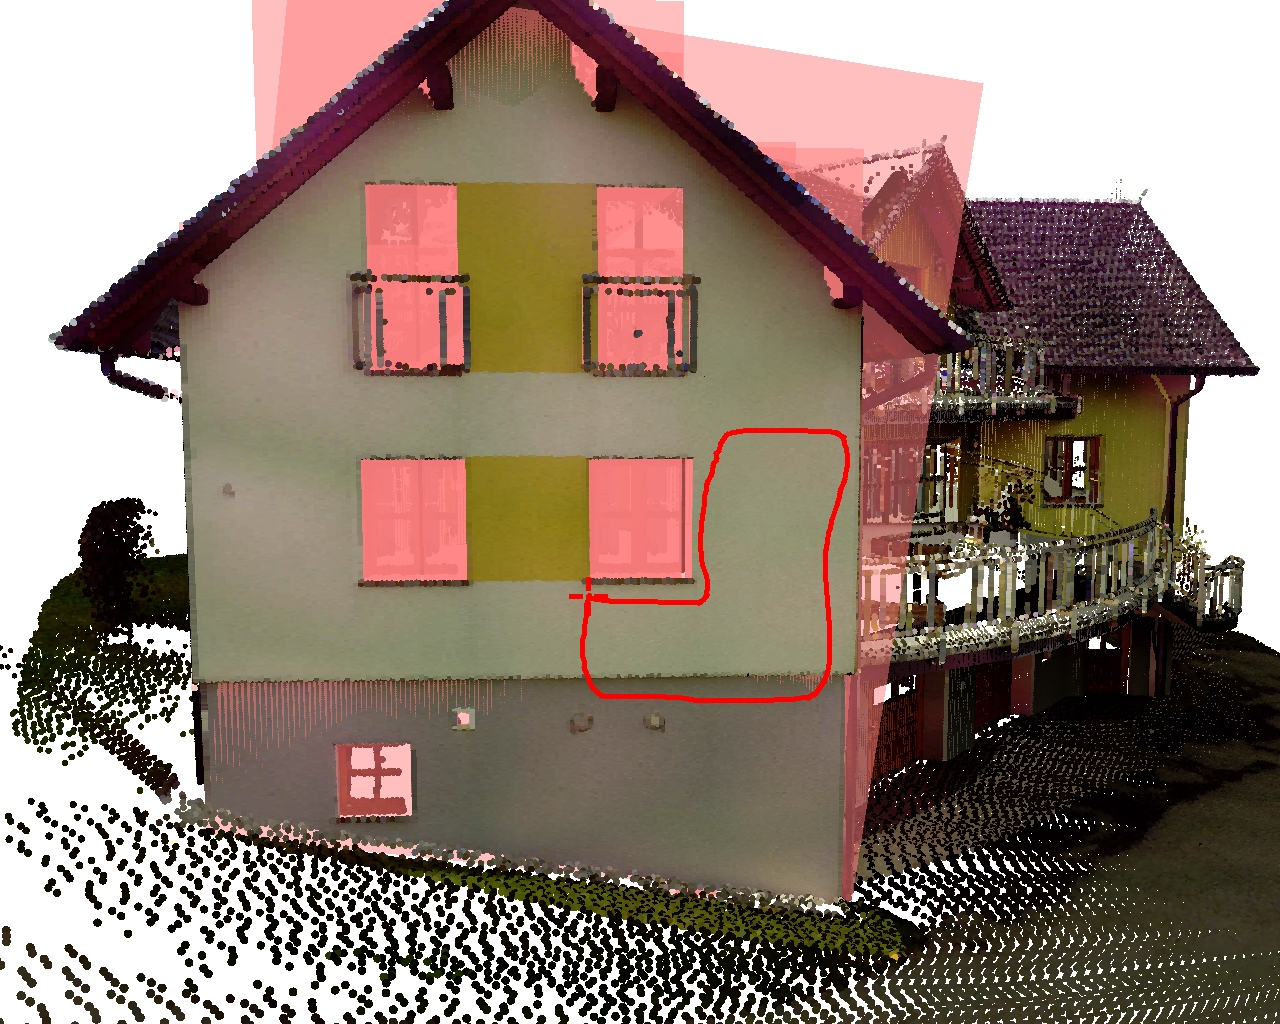
\includegraphics[width=0.5\textwidth]{System_Design/lasso_assisted1.png}%7
	}\par\medskip
	\subcaptionbox{ \label{fig:lasso_assisted2}}{%
		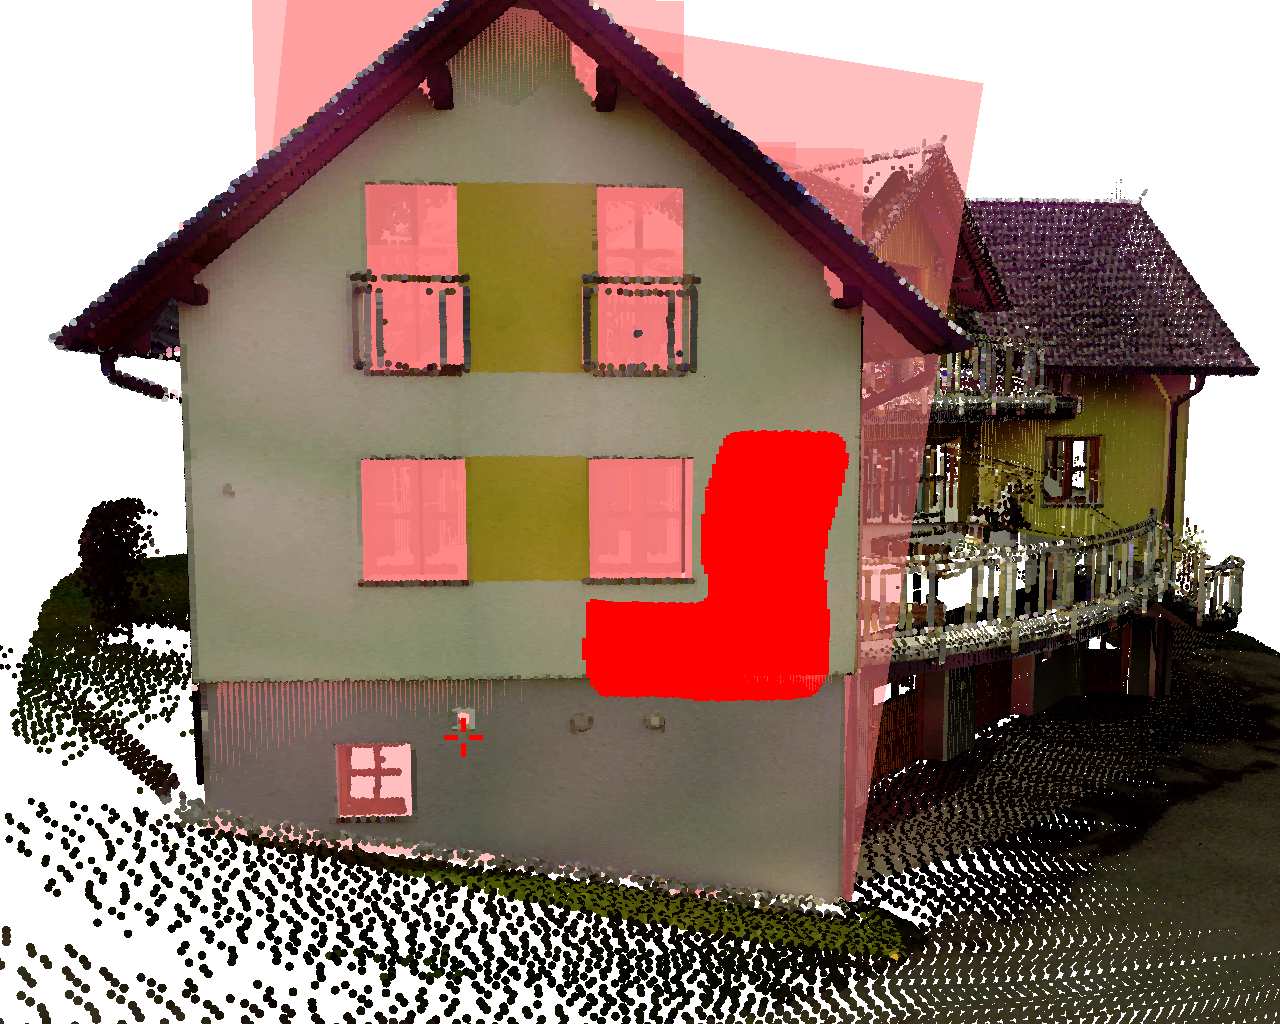
\includegraphics[width=0.5\textwidth]{System_Design/lasso_assisted2.png}%
	}\par\medskip        
	\subcaptionbox{ \label{fig:lasso_assisted3}}{%
		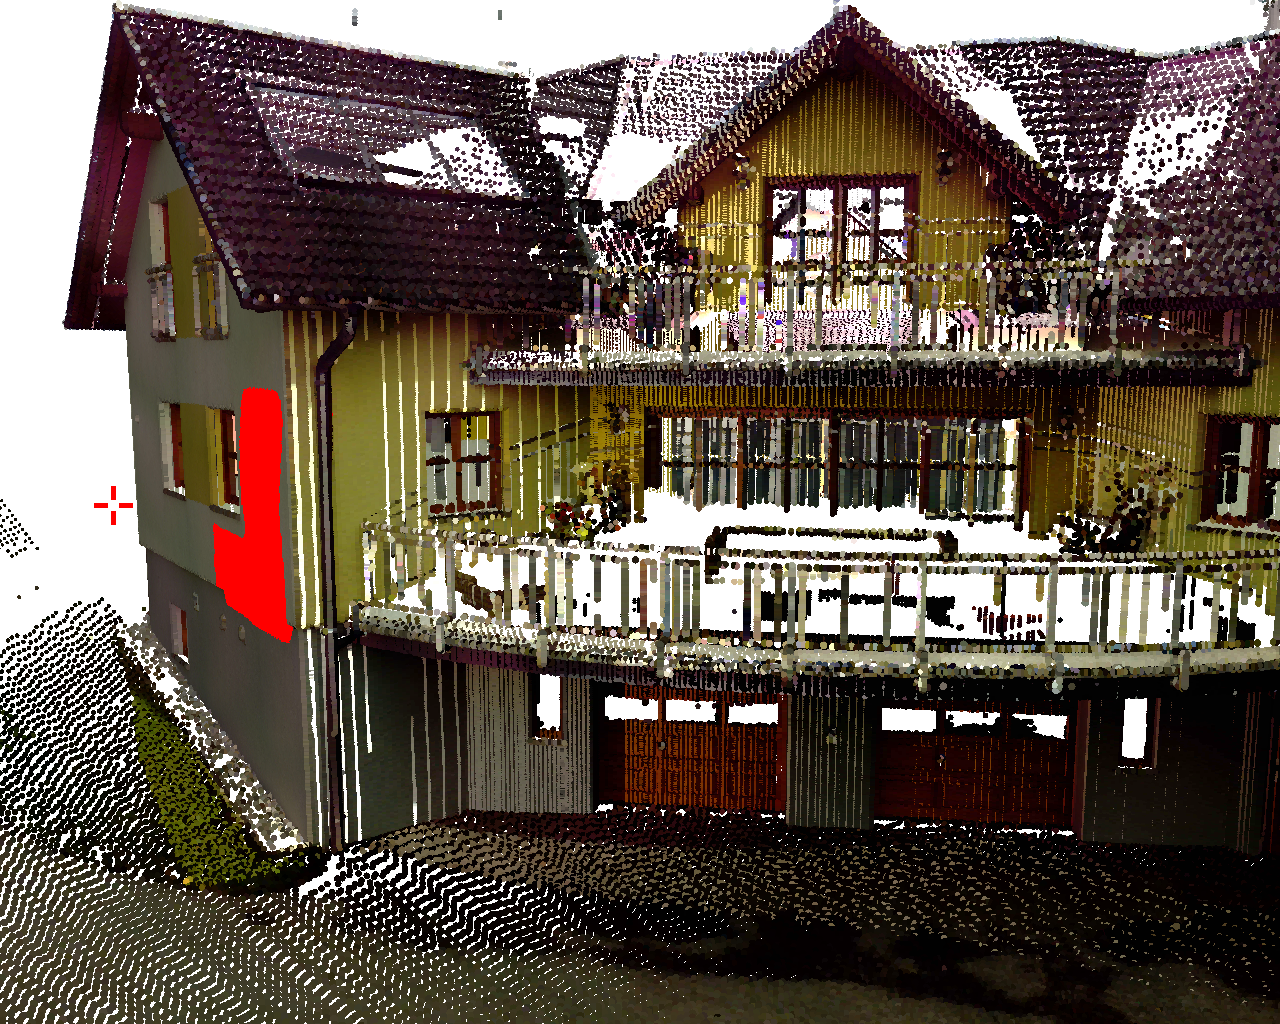
\includegraphics[width=0.5\textwidth]{System_Design/lasso_assisted3.png}%
	}
	\caption[Screenshots of the workflow of a shape-assisted lasso selection. (a) shows the lasso and the support shape, (b) the selected points, (c) shows that only points are selected on the support shape.]
	{(a) - (c) show a \textit{shape-assisted lasso selection} performed on a point cloud. The front-facing wall is selected as support shape by the user. The shape cluster is visualized in light red. In (a) the user draws a polygon on the screen after selecting a shape as support shape. (b) shows the selected points visualized in red from the same point of view. Upon view change, it can be seen that this interaction only selects points that belong the shape cluster. }
	\label{fig:lasso_assisted}
\end{figure}


\subsubsection{Volumetric Brush}

The \textit{volumetric brush} \cite{weyrich2004post, scheiblauer2011out} is designed in such a way that a volume is projected onto the foremost geometry. Points that intersect this volume are considered to be selected. To retrieve the projected position of the volume (e.g., a sphere) the depth buffer is consulted, and the depth value for the current mouse position is retrieved. The world position is the unprojection of the mouse position's $xy$-coordinates and the depth value. 

Since this technique follows the foremost geometry only, sudden depth changes occur if different geometry occludes the area of interest. Thus, view changes are still required to achieve the example task. In regions close to intersections with other structures, such as below the roof, the user must control the size of the volume to not select points on neighboring structures. 


\subsubsection{Shape-Assisted Volumetric Brush}

The \textit{volumetric brush} can easily be adapted to be used in combination with support shapes. Instead of consulting the depth buffer to reconstruct the cursor’s world position, the pick ray is intersected with the selected support shape, thus resulting in a three-dimensional world position. The octree is consulted for nodes that intersect the support shape and the sets of points are reduced to only those that are approximated by the support shape. 
Figure \ref{fig:brush} shows a \textit{Shape-Assisted Volumetric Brush} interaction performed on a wall. The wall creates as a cluster of planes. Only points are selected that belong to this cluster. 

\begin{figure}
	\centering
	\subcaptionbox{ \label{fig:brush_assisted1}}{%
		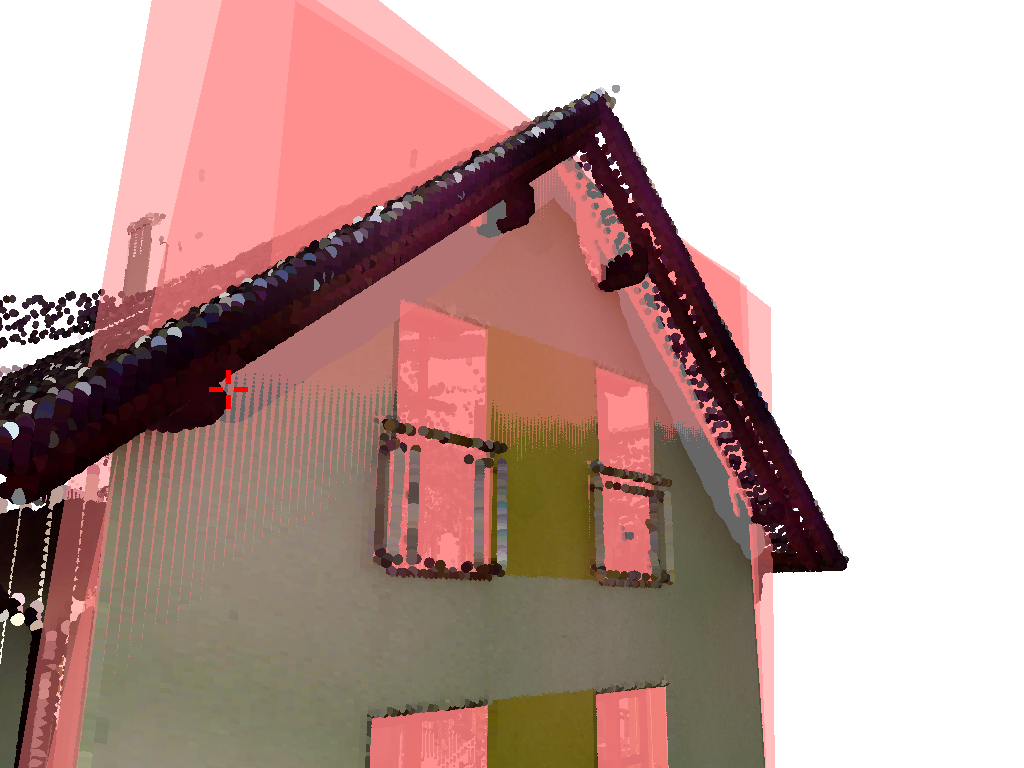
\includegraphics[width=0.8\textwidth]{System_Design/brush1.png}%7
	}\par\medskip
	\subcaptionbox{ \label{fig:brush_assisted2}}{%
		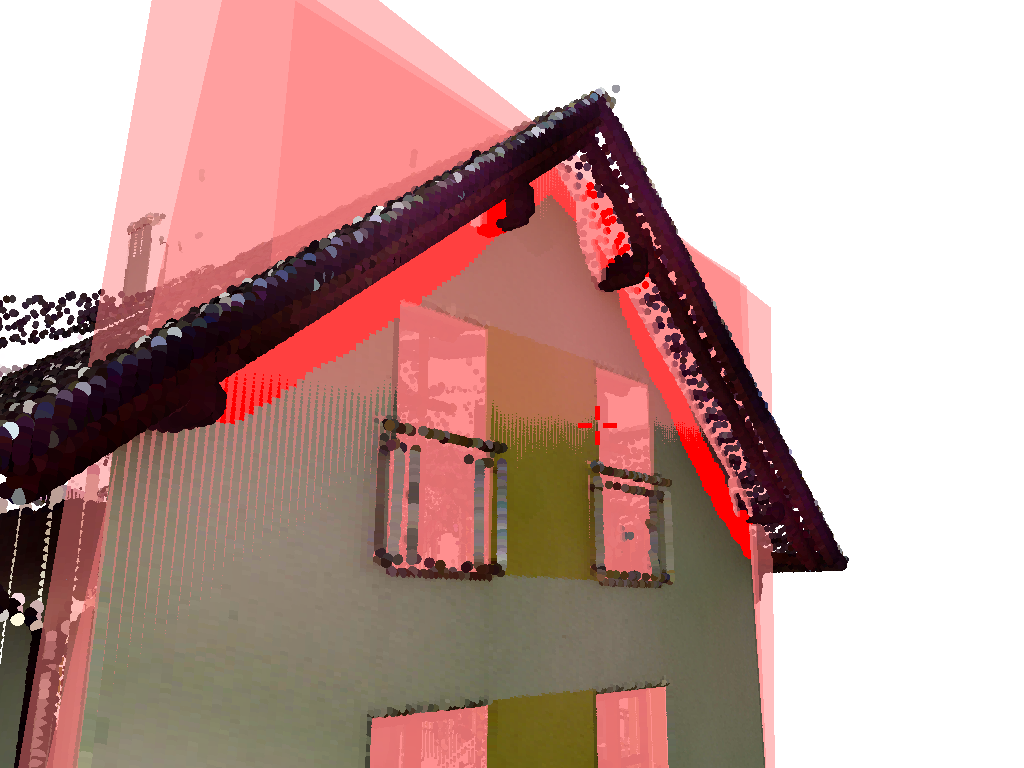
\includegraphics[width=0.8\textwidth]{System_Design/brush2.png}%
	}
	\caption[Workflow of the shape-assisted volumetric brush. (a) shows the trajectory of the brush, (b) shows the selected points. ]
	{This figure shows a \textit{shape-assisted volumetric brush} selection performed shape cluster (transparent red) detected in a point cloud. In (a) the trajectory of the brush is shown as subsequently rendered spheres(grey). (b) shows the selected points for this brush interaction. Even tough some points of the roof structure are intersecting the brush, they are not selected. }
\label{fig:brush}
\end{figure}


\subsection{Shape-Assisted Local Level-of-Detail Increment}
\label{sec:lod_increment}
	
To further investigate the local structures of a point cloud, the currently rendered maximum level-of-detail might not suffice. The highest level of detail is chosen such that the GPU is not overloaded and the balance between detail and performance is retained. Temporarily adding a handful of additional nodes is sufficient to provide more detailed information, and does not pose an enormous impact on performance. 
	
\par
	
Section \ref{sec:renderHorizon} describes a cut in the octree that separates the rendered from the unrendered parts of the point cloud. Furthermore, it introduces the border set, a set of nodes that are rendered, but one of their children is not anymore. A raycast is performed on the border set, resulting in a first set of candidate nodes. The successor nodes of the candidate nodes hold more detailed information on the region of interest that can be accessed easily. Depending on a user-controlled \textit{level-of-increment} parameter, the successors of these nodes are added to the scene and rendered. A \textit{level-of-increment} value of $1$ results in adding only the children, a parameter of $2$ results in adding all children's children, ignoring the nodes in-between, to the scene. 
By adding smaller nodes of higher level-of-detail, the overall detail in the scene is amplified. However, by plainly adding additional nodes, noise and unwanted structures are amplified as well. 

\par
	
\textit{Shape-assisted local level-of-detail increment} utilizes a selected shape cluster to amplify detail only on structures of interest. The user selects a primitive shape as support shape. Instead of performing a raycast, the nodes on the render horizon that intersect the support shape are collected. From these nodes, only those points that are approximated by the support shape are added to the scene. 
	
	\begin{figure}
		\centering
		\subcaptionbox{ \label{fig:lod_increment1}}{%
			\includegraphics[width=0.8\textwidth]{System_Design/lod_Increase.png}%7
		}\par\medskip
		\subcaptionbox{ \label{fig:lod_increment2}}{%
			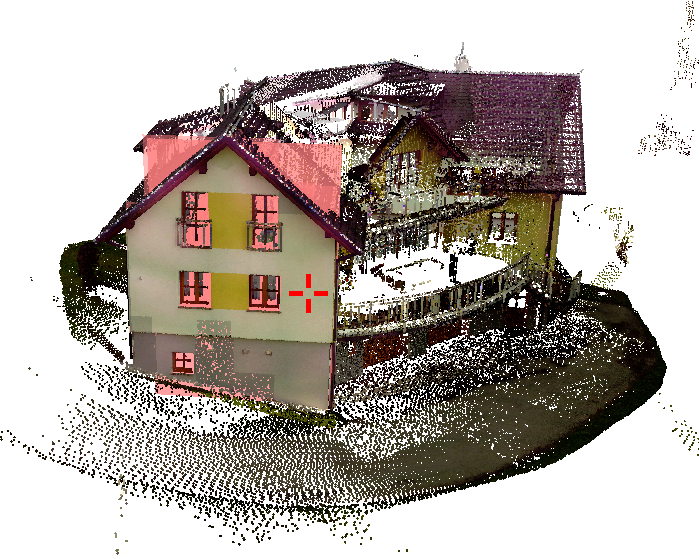
\includegraphics[width=0.8\textwidth]{System_Design/lod_Increase2.png}%
		}
		\caption[Comparison of a scene with and without shape-assisted level-of-detail increment.]
		{This figure shows the benefits of \textit{shape-assisted level-of-detail increment} for a point cloud. (a) shows the currently rendered structure, as well as as shape cluster that is currently selected (red). (b) shows the scene with amplified details along the structure. The additional points are rendered without lighting to appear brighter.}
		\label{fig:lod_increment}
	\end{figure}
	
	Figure \ref{fig:lod_increment} showcases the difference in a scene with and without amplified details along a wall. The selected support shape is rendered in transparent red, while the additional points are rendered without lighting to appear brighter. In the intersecting octree nodes, only those points are rendered that fulfill the shape's score function. 
	
	
